\documentclass[a4paper,12pt]{amsart}
\usepackage{amssymb,amsmath}
\usepackage{tikz}
\usetikzlibrary{calc,fadings,arrows.meta,decorations.pathreplacing}

\begin{document}

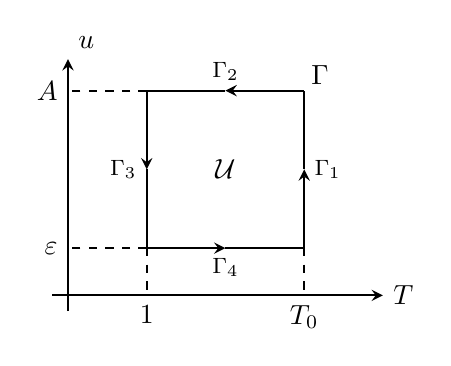
\begin{tikzpicture}[>=stealth,thick]
  \coordinate (a) at (1,0. 6);
  \coordinate (b) at (3,0. 6);
  \coordinate (c) at (1,2. 6);
  \coordinate (d) at (3,2. 6);

  \draw[->] (-0. 2,0) --  (4,0) node[right] {$T$};
  \draw[->] (0,-0. 2) -- (0,3) node[above right] {$u$};

  \draw[->] (a) -- (2,0. 6) node[below] {\footnotesize $\Gamma_4$};
  \draw (2,0. 6) -- (b); 
  \draw[->] (b) -- (3,1. 6) node[right] {\footnotesize $\Gamma_1$};
  \draw (3,1. 6) -- (d); 
  \draw[->] (d) -- (2,2. 6) node[above] {\footnotesize $\Gamma_2$};
  \draw (2,2. 6) -- (c); 
  \draw[->] (c) -- (1,1. 6) node[left] {\footnotesize $\Gamma_3$};
  \draw (1,1. 6) -- (a); 

  \draw[dashed] (a) -- (1,0) node[below] {$1$};
  \draw[dashed] (b) -- (3,0) node[below] {$T_0$};
  \draw[dashed] (a) -- (0,0. 6) node[left] {$\varepsilon$};
  \draw[dashed] (c) -- (0,2. 6) node[left] {$A$};

\node at (2,1. 6) {$\mathcal{U}$};
\node at (3. 2,2. 8) {$\Gamma$};
\end{tikzpicture}

\end{document}